\chapter{Ground Vibration Testing}
\label{ch:gvt}

Ground vibration testing (GVT) was performed to validate the finite-element model of MARGE. The frequency responses of accelerometers to an impulse input were generated from the experimental data. Using these, the natural frequencies and the damping ratios of dynamic modes of the system were determined.

Two sets of data were collected. The first set of data was collected with the model as designed, including the rigid-body pitching mode. This data was used to determine the damping ratios of the modes. The second set of data was collected with the root of the MARGE wing clamped to eliminate the rotational rigid-body mode. This was done to enable data acquisition of flexible-body modes without exciting and losing energy to the rigid-body mode. This data was used to tune the finite-element model and to determine the damping ratios of the wing bending modes.

%%%%%%%%%%%%%%%%%%%%%%%%%%%%%%%%%%%%%%%%%%%%%%%%%%%%%%%%%%%%%%%%
\section{Test Setup} %%%%%%%%%%%%%%%%%%%%%%%%%%%%%%%%%%%%%%%%%%%
%%%%%%%%%%%%%%%%%%%%%%%%%%%%%%%%%%%%%%%%%%%%%%%%%%%%%%%%%%%%%%%%

The equipment used for the test include:
\begin{itemize}
    \item PCB Piezotronics ICP Impact Hammer Model 086C03
    \item PCB Piezotronics ICP Accelerometer Model 352C22
    \item National Instruments Breakout <insert>
    \item National Instruments DAQ Module <insert>
\end{itemize}

The impact hammer and accelerometers were connected to the DAQ system which was connected to a personal computer. The computer recorded data from the DAQ system using the Data Acquisition Toolbox in MATLAB software.

%---------------------------------------------------------------
\subsection{Sensor Placement}
%---------------------------------------------------------------

The accelerometers were placed in locations such that all of the flexible modes of interest were observable. This was done by placing accelerometers near anti-nodal points of the modes as predicted by the finite-element model. The accelerometer locations for the two sets of testing are shown in Fig. \ref{fig:accelPlacement}

\begin{figure}[h]
    \centering
    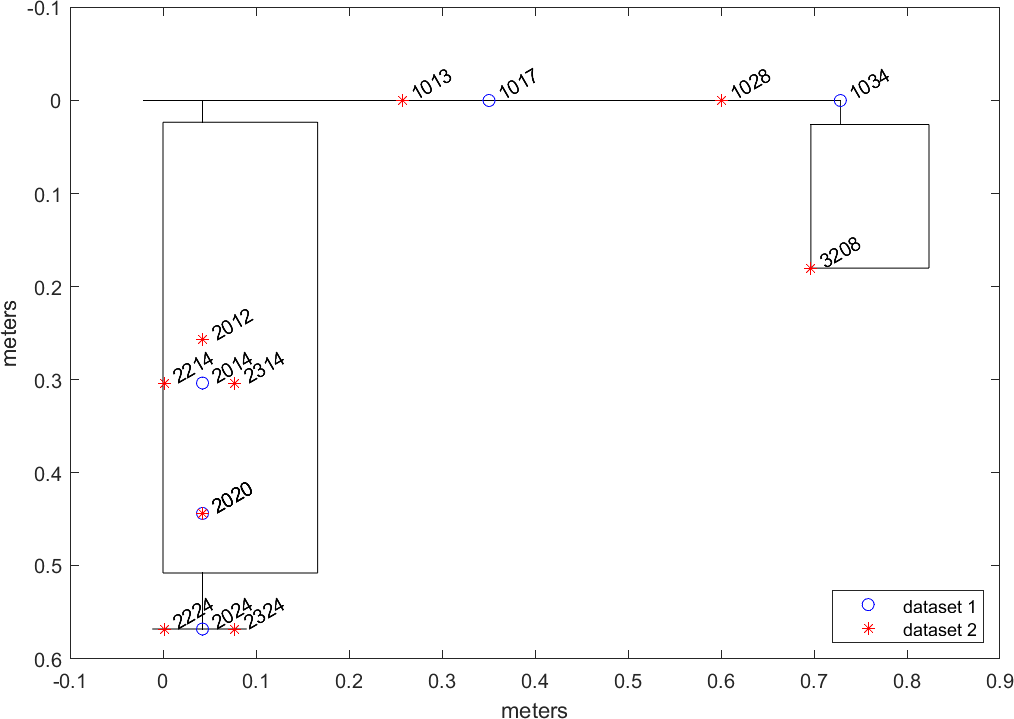
\includegraphics[width=4in]{figs/GVT/accelLocPlot.png}
    \caption{Accelerometer placement in ground vibration testing of MARGE}
    \label{fig:accelPlacement}
\end{figure}

The impact hammer hits were also placed at these same locations on the structure as the accelerometers.

For the second dataset, pairs of accelerometers on the wing located a short distance apart chordwise were also treated as a fictional third accelerometer by taking their difference. This was done to create a sensor observing only torsional modes of the wing.

%%%%%%%%%%%%%%%%%%%%%%%%%%%%%%%%%%%%%%%%%%%%%%%%%%%%%%%%%%%%%%%%
\section{Generating Frequency Response Functions} %%%%%%%%%%%%%%
%%%%%%%%%%%%%%%%%%%%%%%%%%%%%%%%%%%%%%%%%%%%%%%%%%%%%%%%%%%%%%%%

Each GVT test point (input-output combination) was post-processed to generate the frequency response functions (FRFs) of the accelerometers to the impacts. This section describes the steps in this process.

The time-series data was truncated to to start just before the impulse input and end after $t$ seconds (where $t$ is chosen so that the data is long enough to characterize the lowest frequency of interest). This was done to isolate the portion of the data with a good signal-to-noise ratio.

Each test point was recorded as three (in the second dataset) or five (in the first dataset) separate impacts. After truncation, the signals from these impacts were concatenated to form one continuous time-domain signal. The mean of this combined signal was then subtracted from it so that there would be no steady-state component in the frequency response.

This signal was then buffered into overlapping segments and transformed using a chirp z-transform (CZT). The CZT is a function which computes power spectra from time-domain signals. It has an advantage over the similar discrete Fourier transform (DFT) in that it has the ability to increase the resolution of the transformed response in the bandwidth of interest. The purpose of first buffering the signal is to reduce the effect of noise.

The products of the CZT are the power spectra of the signals. For any given accelerometer power spectrum $S_y$ and impact hammer power spectrum $S_x$, the frequency response function can then be computed as
\begin{align}
    FRF &= \frac{G_{yy}}{G_{yx}}
\end{align}
where
\begin{align}
    G_{yx} &= S_y^* \cdot S_x \\
    G_{yy} &= |S_y|^2 \\
\end{align}
The coherence can also be computed as
\begin{align}
    \frac{|G_{xy}|^2}{|G_{xx}||G_{yy}|}
    % (abs(Gxy_hat).^2)./(abs(Gxx_hat).*abs(Gyy_hat))
\end{align}
\begin{align}
    G_{xy} &= S_x^* \cdot S_y \\
    G_{yy} &= |S_y|^2 \\
\end{align}

The frequency response functions computed for the GVT data are shown in Appendix \ref{ch:appendix}.

%%%%%%%%%%%%%%%%%%%%%%%%%%%%%%%%%%%%%%%%%%%%%%%%%%%%%%%%%%%%%%%%
\section{Determining Modal Properties} %%%%%%%%%%%%%%%%%%%%%%%%%
%%%%%%%%%%%%%%%%%%%%%%%%%%%%%%%%%%%%%%%%%%%%%%%%%%%%%%%%%%%%%%%%

Once the FRFs were computed, the natural frequencies and damping of the modes are determined from the FRFs.

The natural frequencies were computed manually as the max magnitude of the response at the peaks.

The frequency 